\begingroup
\setlength{\emergencystretch}{1.5em}
\section{Evaluation}
\label{sec:evaluation}
In the tables, LSAA denotes the reference configuration using the native task-specific heads together with shared \texttt{C-W} supervision across tasks. All results are reported as percentages and are compared with percentage points for scores, with each value representing the mean performance across three seeds and the corresponding sample standard deviation shown as a subscript. Where applicable, bold and underlined entries indicate the highest and second-highest mean values, respectively, to facilitate comparison across methods and configurations.

For ICBHI cycles, Score is $(Sp+Se)/2$, where specificity $Sp$ is Normal recall and sensitivity $Se$ is the fraction of all abnormal cycles assigned their correct Crackle, Wheeze, or Both class\cite{rocha2019icbhi}. For SPRSound events, Score is $(AS+HS)/2$, where average score $AS=(r_N+r_A)/2$ and harmonic score $HS=2r_Nr_A/(r_N+r_A)$ use Normal recall $r_N$ and Adventitious recall $r_A$; $HS=0$ when both recalls are zero\cite{zhang2022sprsound}. HF uses recording-level area under the receiver operating characteristic curve (AUROC): recordings with Wheeze, Rhonchi, or Stridor annotations are positive, and other eligible recordings form the Other class, which does not denote Normal. We evaluate 957 HF test recordings with adventitious-sound annotations (661 positive and 296 Other); phase-only and unannotated recordings are excluded. KAUH uses patient-level balanced accuracy (BA)~\cite{brodersen2010balanced}, the mean Normal/Abnormal recall after aggregating filter-version probabilities.

\subsection{Joint Learning and Cross-Dataset Transfer}
\vspace{2mm}
\label{sec:protocol}
\label{sec:native_results}
\emph{One joint model supports both native tasks with competitive transfer performance} (Table~\ref{tab:native_results}). LSAA exceeds every frozen-encoder reference~\cite{niizumi2025foundationeval,niizumi2025m2dresp} in mean ICBHI Score, HF AUROC, and KAUH BA, while its SPRSound Score of 90.86 points is 0.69 points below the strongest reference, BEATs. Encoder fine-tuning also differs from the frozen references~\cite{niizumi2025foundationeval}, so these gains reflect the complete system; the ablations examine shared supervision more directly.

\LSAAMainResultsTable
\vspace{2mm}
The multilabel adaptations show that advantages depend on the evaluation target (Table~\ref{tab:system_comparison}). \emph{LSAA has the highest mean ICBHI Score, HF AUROC, and KAUH BA}, whereas DCASE leads on SPRSound. DCASE shares a union of native classes, while LSAA combines shared \texttt{C-W} supervision with separate native task heads. However, DCASE uses frozen BEATs with a trainable convolutional recurrent network, while LSAA fine-tunes the encoder. PC-MCL trains only on ICBHI, making its SPRSound result a cross-source comparison. These system differences prevent attributing the rankings to label representation alone.

\LSAASystemComparisonTable
\subsection{Supervision Analysis and Ablation Study}
\label{sec:ablations}
\label{sec:transfer}
\vspace{2mm}
% \begin{figure}[!htbp]
% \centering
% 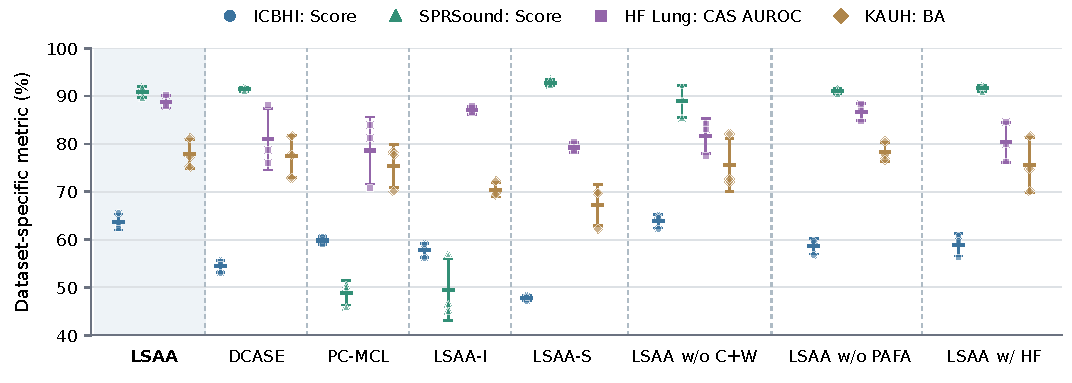
\includegraphics[width=\columnwidth]{Figure/figure3_unified_seed_performance.pdf}
% \caption{Performance of LSAA, comparison systems, and ablation variants across four datasets.}
% \label{fig:performance_comparison}
% \end{figure}

The single source models have limited cross-dataset task coverage (Table~\ref{tab:ablations}). LSAA-I achieves SPRSound Score of 49.53 points, while LSAA-S achieves an ICBHI Score of 47.75 points. Their limited cross source performance motivates sharing supervision across datasets, addressing the transfer question raised by Figures~\ref{fig:dataset_characteristics}~(b) and~(c).

\LSAAAnalysisTable
\vspace{2mm}
\label{sec:fine_supervision}
\label{sec:readout_analysis}
\emph{Shared \texttt{C-W} supervision supports native prediction and external transfer. }LSAA w/o \texttt{C-W} retains the native task heads but removes the auxiliary \texttt{C-W} losses. Compared with this variant, LSAA improves mean SPRSound Score by \textbf{1.93 points}, HF AUROC by \textbf{7.16 points}, and KAUH BA by 2.32 points, with a 0.20 points ICBHI Score decrease. Fine-grained labels can therefore support a binary native task and external transfer while largely preserving ICBHI performance. The HF improvement occurs in all three seeds, while SPRSound and KAUH improve in two. Both models use fixed readout rules over their ICBHI native heads for external evaluation. The gains therefore show that \emph{shared attribute supervision can benefit predictions produced through a native task head which supports using annotation detail to guide shared representation learning while allowing each task to retain its own prediction interface.}

Native and transfer performance show different rankings in the PAFA comparison. LSAA has a 5.07 points higher ICBHI Score than LSAA w/o PAFA, while its KAUH BA is 0.39 points lower. Higher native-task performance does not necessarily coincide with stronger external transfer.

\label{sec:hf_supervision}
Additional HF supervision does not yield stronger performance. Relative to LSAA, LSAA w/HF has a mean SPRSound Score that is 0.76 points higher, but lower ICBHI Score, HF AUROC, and KAUH BA by 4.77 points, 8.47 points, and 2.40 points, respectively. HF supervision yielded no gains under the current mapping and weighting, suggesting a need to better align annotation semantics and sampling across datasets.
\par
\endgroup
